\subsection{Analyse der blauen $\sigma$-Linien}
<<<<<<< HEAD
Vollkommen analog wird die $\sigma$-Aufspaltung des blauen Lichtes analysiert.
Die Aufspaltung der blauen Spektrallinie ist in \autoref{fig: aufspaltung_blau_sigma} dargestellt.
Gemäß Formel~\eqref{eq: fitfuntion_hysterese}
=======
Vollkommen analog wird die $\sigma$-Aufspaltung des blauen Lichtes analysiert. % Vollkommen klingt als Einleitung nicht so schön
Die Aufspaltung der blauen Spektrallinie ist in Abbildung \ref{fig: aufspaltung_blau_sigma} dargestellt.
Gemäß Formel \eqref{eq: fitfuntion_hysterese}
>>>>>>> kommentare
führt der anliegende Spulenstrom von $I = \SI{10}{\ampere}$ zu einer magnetischen Feldstärke von $B = \SI{346(3)}{\milli\tesla}$.

Die Helligkeit in Abhängigkeit von der horizontalen Position auf den aufgenommenen Bildern ist in \autoref{fig: blau_intensität_sigma} für das unaufgespaltene
und aufgespaltene Beugungsbild dargestellt. Anhand dessen werden die Positionen von $10$ Intensitätsmaxima und ihrer Aufspaltungen
vermessen. Die Daten sind in \autoref{tab: peaks_blau_sigma} aufgeführt.
Eine graphische Darstellung der abgelesenen Intensitätsmaxima befindet sich in den Abbildungen~\ref{fig: peaks_blau_0}
und~\ref{fig: peaks_blau_sigma_6}.

Die für die Berechnung der Wellenlängenänderung relevanten Abstände $\Delta s_i$ und $\delta s_i$
sind in \autoref{tab: abstände_blau_sigma}
aufgeführt. Mit Hilfe der Gleichungen~\eqref{} berechneten Größen sind in Tabelle
\ref{tab: abstände_blau_sigma} eingetragen. Als Mittelwert für den Landé-Faktor ergibt sich
\begin{equation}
  g = \num{2.02(2)}.
\end{equation}
\begin{figure}
  \centering
  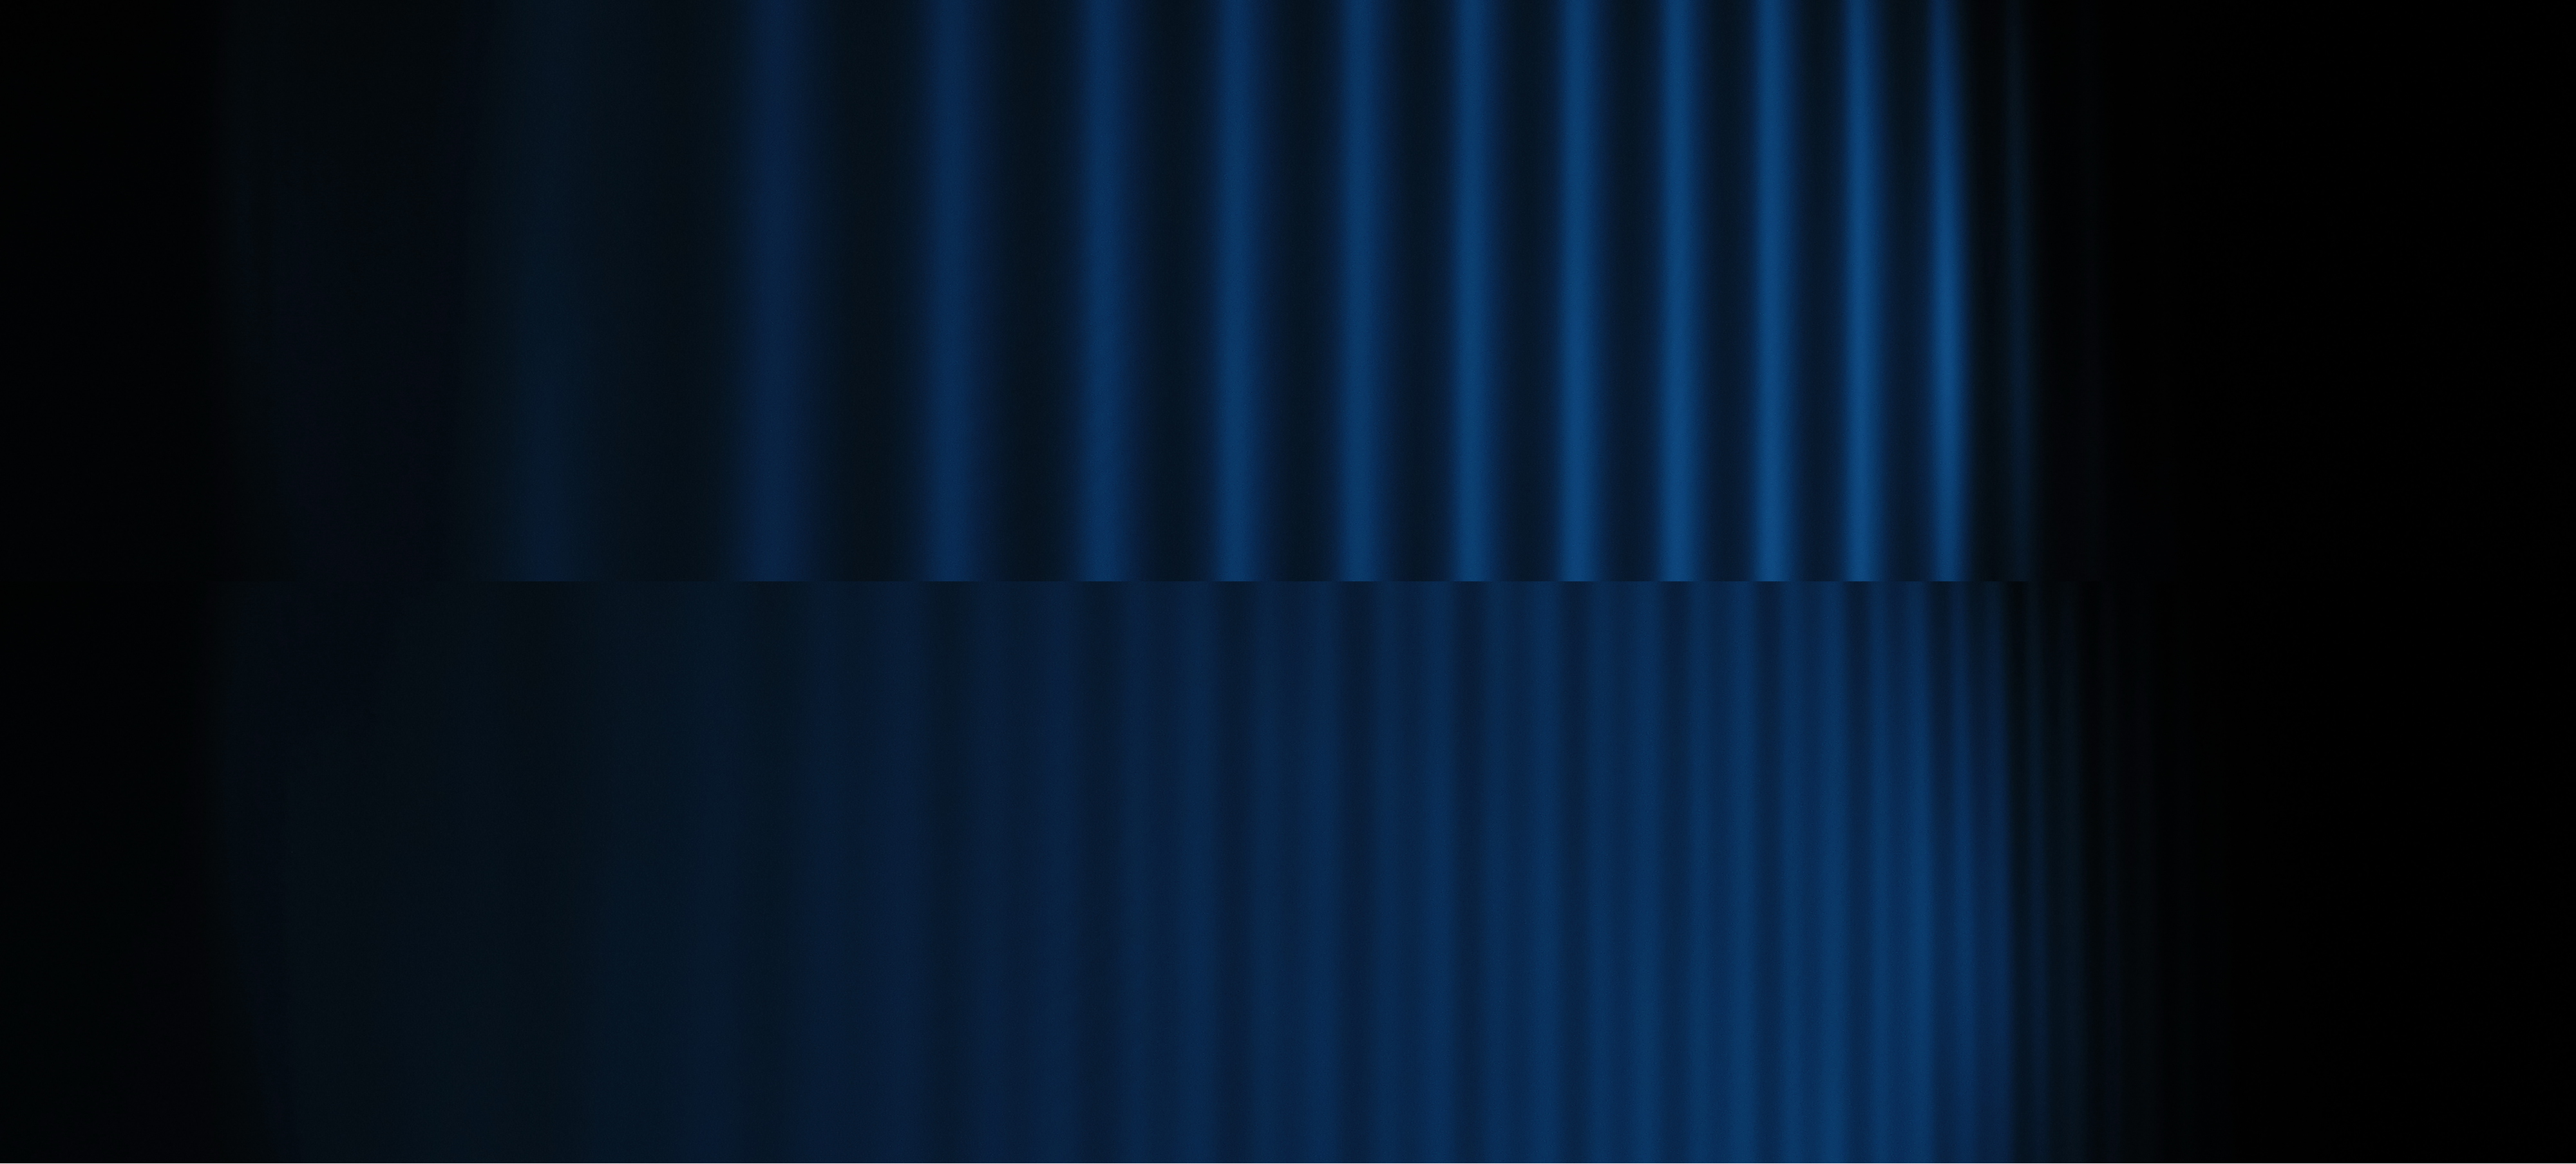
\includegraphics[width = 0.7\textwidth]{../Messdaten/bilder_v27/messung_2_blau_sigma/aufspaltung_blau_sigma.png}
  \caption{Blau $\sigma$: Aufgenommene Intensitätsstreifen des blauen Lichtes (von oben nach unten) $\SI{0}{\ampere}$ und $\SI{6}{\ampere}$ Feldstrom.}
  \label{fig: aufspaltung_blau_sigma}
\end{figure}
\begin{figure}
  \centering
  \includegraphics[width = 0.7\textwidth]{../Messdaten/plots/blau_sigma_intensitaet.pdf}
  \caption{Blau $\sigma$: Darstellung der Helligkeit der blauen Linien in Abhängigkeit von der horizontalen Lage auf dem Foto.}
  \label{fig: blau_intensität_sigma}
\end{figure}
\begin{table}
\centering
\caption{Blaue Sigma Aufspaltung: Positionen $x_0$ und $x_{6}$ der Intensitätsmaxima unter $I= \SI{0}{\ampere}$ und $I= \SI{6}{\ampere}$.}
\label{tab: peaks_blau_sigma}
\begin{tabular}{S S[table-format=4.0] S[table-format=4.0] } 
\toprule
{$x_0 / $px} & \multicolumn{2}{c}{$x_{6} \:/\: $px} \\
\midrule
1483 & 1408 & 2402\\
1708 & 1539 & 2487\\
1909 & 1641 & 2555\\
2121 & 1759 & 2641\\
2285 & 1859 & 2702\\
2449 & 1967 & 2788\\
2605 & 2051 & 2843\\
2752 & 2154 & 2930\\
2891 & 2235 & 2985\\
3030 & 2320 & 3052\\
\bottomrule
\end{tabular}
\end{table}

Eine graphische Darstellung der abgelesenen Intensitätsmaxima befindet sich in den Abbildungen \ref{fig: peaks_blau_0} und \ref{fig: peaks_blau_sigma_6}. % Doppelter Zeilenabstand vor Eine
\begin{figure}
  \centering
  \includegraphics[width = 0.7\textwidth]{../Messdaten/plots/peaks_blau_sigma_0.pdf}
  \caption{Darstellung der abgelesenen Lagen der Intesitätsmaxima für das Beugungsbild unter $I =\SI{0}{\ampere}$.}
  \label{fig: peaks_blau_0}
\end{figure}
\begin{figure}
  \centering
  \includegraphics[width = 0.7\textwidth]{../Messdaten/plots/peaks_blau_sigma_6.pdf}
  \caption{Blau $\sigma$: Darstellung der abgelesenen Lagen der Intesitätsmaxima für das Beugungsbild unter $I =\SI{6}{\ampere}$.}
  \label{fig: peaks_blau_sigma_6}
\end{figure}
Die für die Berechnung der Wellenlängenänderung relevanten Abstände $\Delta s_i$ und $\delta s_i$ sind in Tabelle \ref{tab: abstände_blau_sigma}
aufgeführt. Mit Hilfe der Gleichungen \eqref{} berechneten Größen sind in Tabelle
\ref{tab: abstände_blau_sigma} eingetragen. Als Mittelwert für den Landé-Faktor ergibt sich %du berechnest doch hier g_ij, dann würde ich den selben Bezeichner verwenden wie in der Anleitun
\begin{equation}
  g = \num{2.02(2)}.
\end{equation}
\begin{table}
\centering
\caption{Blau $\sigma$: Abstände zwichen den unaufgespaltenen Linien $\Delta s_i$ und gemittelte Abstände $\frac{\delta s_i + \delta s_{i+1}}{2}$. Wellenlängenverschiebung $\Delta \lambda$, Energieaufspaltung $\Delta E$ und berechneter Übergangs-Landé-Faktor g.}
\label{tab: abstände_blau_sigma}
\begin{tabular}{S S S S S[table-format=1.2]@{${}\pm{}$} S[table-format=1.2] }
\toprule
{$\Delta s_i / $px} & {$\frac{\delta s_i + \delta s_{i+1}}{2} /$px} & {$\Delta \lambda / \si{ \pico\meter}$} & {$\Delta E / \si{ 10^{-5}\electronvolt}$} & \multicolumn{2}{c}{$g$} \\
\midrule
225 & 124 & 7.5 & 4.0 & 2.00 & 0.02\\
201 & 113 & 7.6 & 4.1 & 2.04 & 0.02\\
212 & 106 & 6.7 & 3.6 & 1.80 & 0.02\\
164 & 94 & 7.7 & 4.2 & 2.08 & 0.02\\
164 & 85 & 7.0 & 3.8 & 1.88 & 0.02\\
156 & 86 & 7.4 & 4.0 & 1.99 & 0.02\\
147 & 86 & 7.9 & 4.2 & 2.12 & 0.02\\
139 & 86 & 8.4 & 4.5 & 2.25 & 0.02\\
139 & 77 & 7.5 & 4.0 & 2.01 & 0.02\\
\bottomrule
\end{tabular}
\end{table}

